\setlength{\columnsep}{3pt}
\begin{flushleft}
	\begin{itemize}
		\item \textbf{kill}: Kills a specific processes by sending some signal to it.
		\begin{tcolorbox}[breakable,notitle,boxrule=-0pt,colback=pink,colframe=pink]
			\color{black}
			\fontdimen2\font=1em
			Syntax: kill [options] [process\_id]
			\fontdimen2\font=4pt
		\end{tcolorbox}
		Eg: Start a process and kill it with it's PID.
			\begin{figure}[h!]
				\centering
				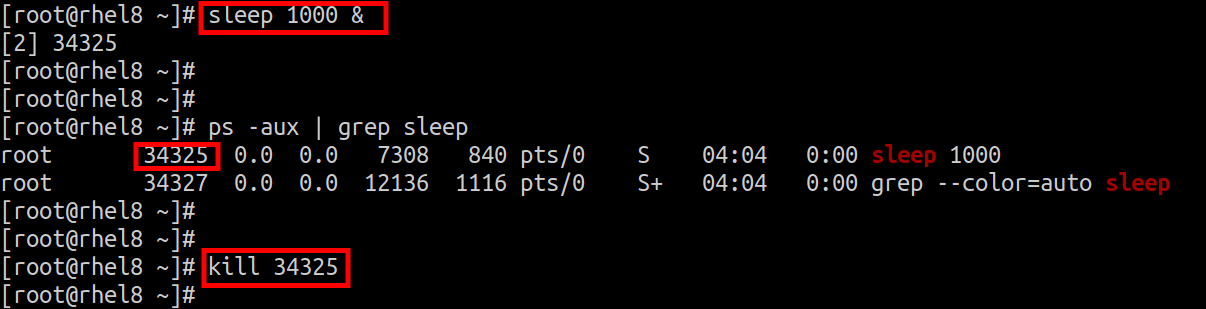
\includegraphics[scale=.3]{content/chapter12/images/kill1.png}
				\caption{Sample output}
				\label{fig:process23482}
			\end{figure}

		
		Options with \textbf{kill} command:	
		\begin{itemize}
			
			\item \textbf{-l}: List all signal associated with kill command.			
			\begin{tcolorbox}[breakable,notitle,boxrule=-0pt,colback=pink,colframe=pink]
				\color{black}
				\fontdimen2\font=1em
				Syntax: kill -l
				\fontdimen2\font=4pt
			\end{tcolorbox}
			Eg: 
			\begin{figure}[h!]
				\centering
				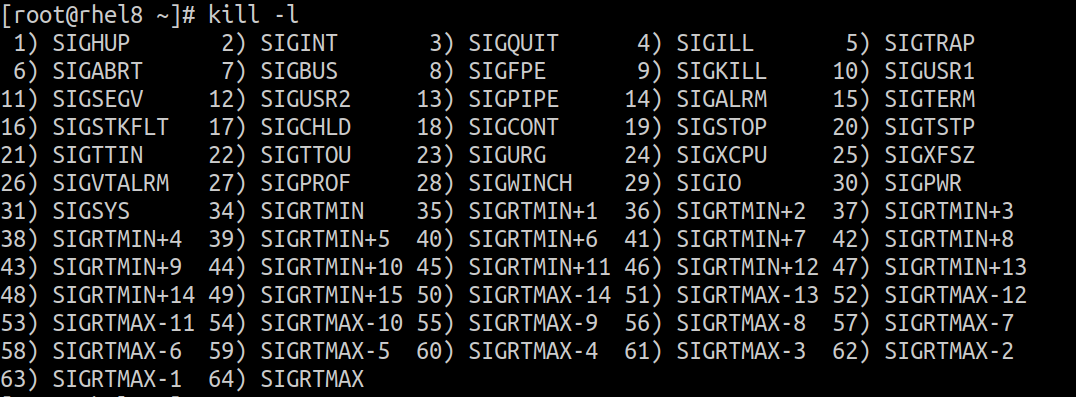
\includegraphics[scale=.3]{content/chapter12/images/kill2.png}
				\caption{Sample output}
				\label{fig:process2347}
			\end{figure}
			\newline
		
			\item \textbf{-signal\_number}: Supply signal while killing a process.
			\begin{tcolorbox}[breakable,notitle,boxrule=-0pt,colback=pink,colframe=pink]
				\color{black}
				\fontdimen2\font=1em
				Syntax: kill -signal\_number process\_id
				\fontdimen2\font=4pt
			\end{tcolorbox}		
			Eg:
			\begin{figure}[h!]
				\centering
				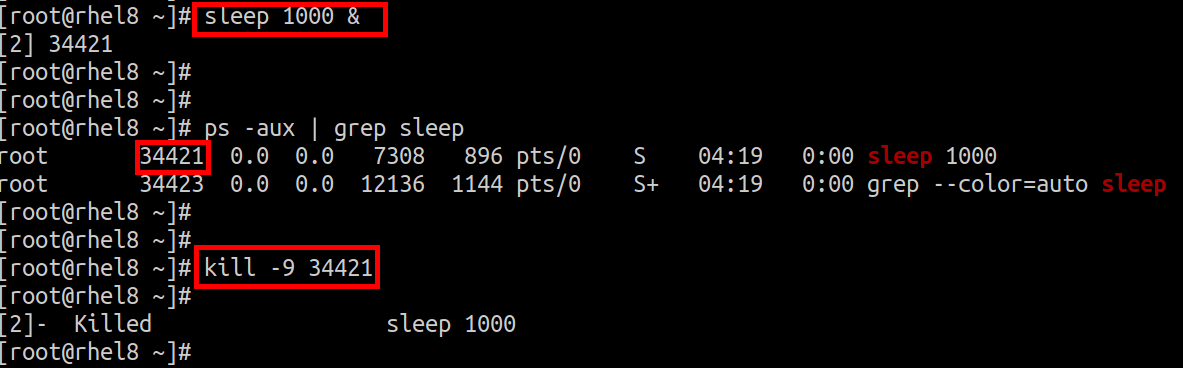
\includegraphics[scale=.25]{content/chapter12/images/kill3.png}
				\caption{Sample output}
				\label{fig:process23456}
			\end{figure}
					
		\end{itemize}
	
	\newpage
	\item \textbf{killall}: Killing any running process by process name instead of it's process ID. Zombie process needs to be killed using process name as they won't have process ID.
	\bigskip
	\begin{tcolorbox}[breakable,notitle,boxrule=-0pt,colback=pink,colframe=pink]
		\color{black}
		\fontdimen2\font=1em
		Syntax: killall [options] process\_name
		\fontdimen2\font=4pt
	\end{tcolorbox}
	Eg:
	\begin{figure}[h!]
		\centering
		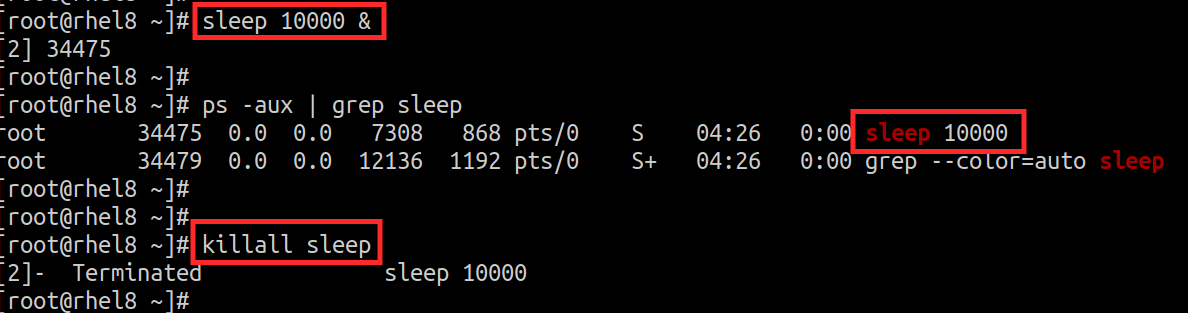
\includegraphics[scale=0.25]{content/chapter12/images/kill4.png}
		\caption{Sample output}
		\label{fig:top_command_output5}
	\end{figure}


		
	\end{itemize}

\end{flushleft}

\newpage


